%% It is just an empty TeX file.
%% Write your code here.

\section{Physics of the Datasets}

% 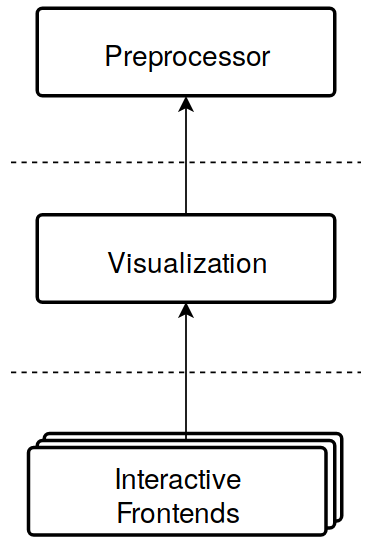
\includegraphics[width=0.8\linewidth]{img/module_design.png}

\begin{frame}\frametitle{How is the data generated?}
    \begin{itemize}

    \item Fleur computes electron density in crystals
    \item Density Functional Theory (DFT) approach:
        \begin{itemize}
        \item Hohenberg-Kohn theorem: use electron density 
        \item Kohn-Sham equations: Solve one particle Schr\"odinger equations in effective potential (self consistent)
        \item State of the art method for electronic structure computations in solids
        \end{itemize}
    \end{itemize}
\end{frame}

\begin{frame}\frametitle{What data is generated?}
    \begin{itemize}
        
        % \item What data is generated?

    \item Bandstructure $E_{\nu}(k)$:
        \begin{itemize}
        \item Eigenenergies of eigenfunctions of the Hamiltonian for each (crystal-) momentum $k$
        \item Dispersion relation: Relation between crystal momentum and energies of the Bloch electrons
        \item Sampled along a 1D path between high symmetry points in 3D reciprocal space 
        \end{itemize}
    \end{itemize}

    \begin{column}{.5\textwidth}
        \begin{figure}
            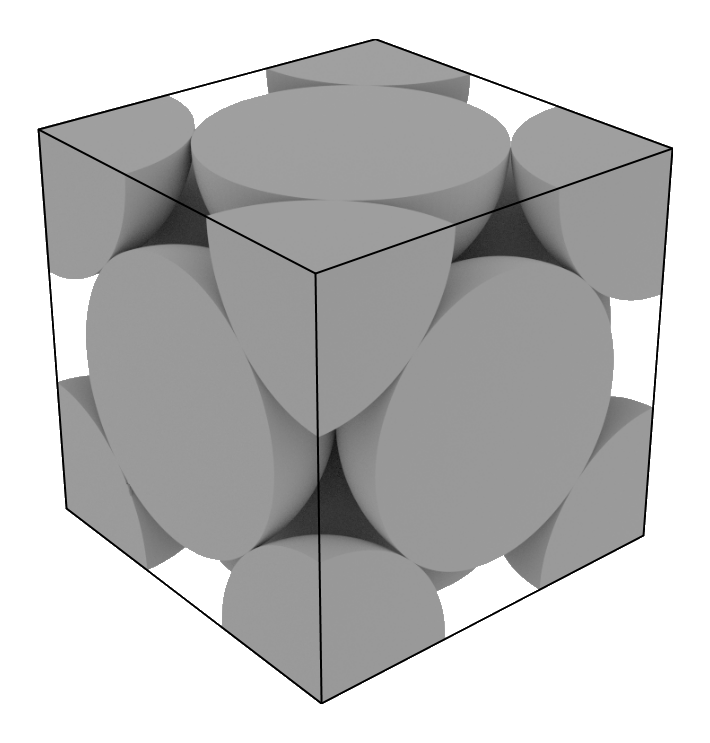
\includegraphics[width=0.7\linewidth]{fig/fcc_real.png}
        \end{figure}

    \end{column}
    \begin{column}{.5\textwidth}
        \begin{figure}
            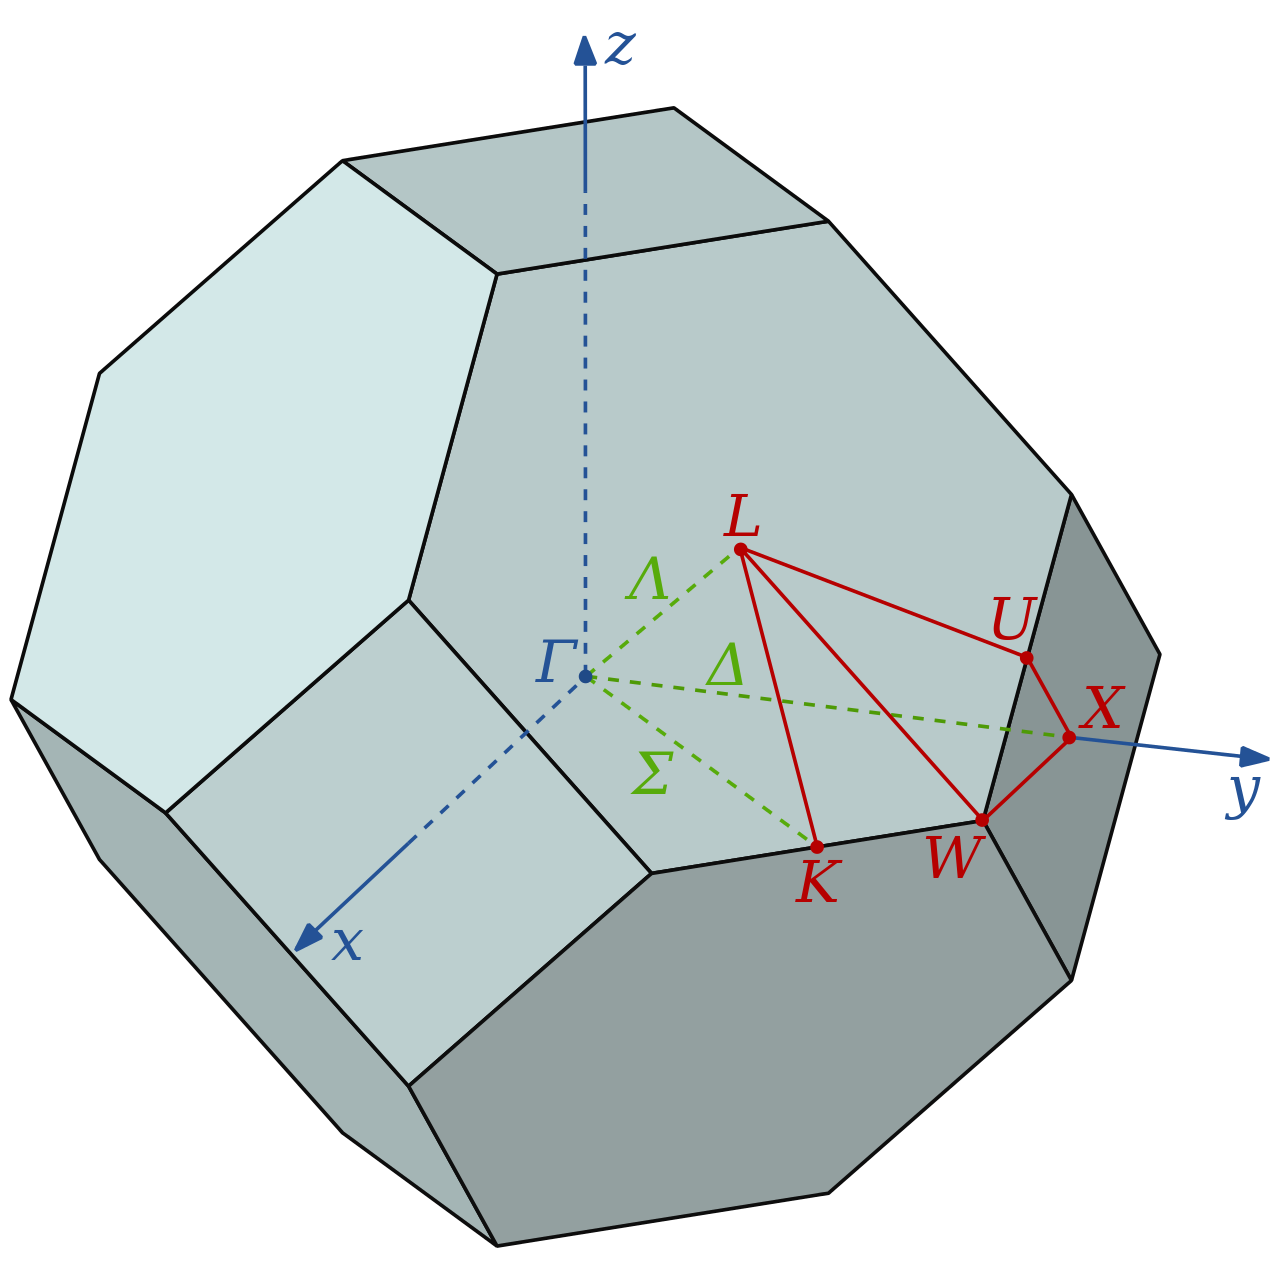
\includegraphics[width=0.7\linewidth]{fig/Brillouin_Zone_(1st,_FCC).png}
        \end{figure}

    \end{column}

    % (Picture fcc real/reciprocal: idea: Schrödinger eqn solved in reciprocal space --> because of translation symmetry...)
\end{frame}

\begin{frame}
    \begin{itemize}
    \item Density of States D(E):
        \begin{itemize}
        \item Density of electron states per energy interval %(k is summed out)
        \end{itemize}

        \
    \item Interesting for physicists: Where do the contributions to E(k) and D(E) come from?
        \begin{itemize}
        \item Contributions from basis functions of the DFT calculation corresponding to different atomgroups and atomic orbitals (s, p, d, f)
        \item User might be interested in any superposition of them (e.g. to locate states in real space)
        \item Information stored in form of weights for all atom groups and the atomic orbitals s, p, d, f 
        \end{itemize}

    \end{itemize}
\end{frame}